\documentclass[10pt,a4paper]{article}
\usepackage[utf8]{inputenc}
\usepackage[english]{babel}
\usepackage{amsmath}
\usepackage{amsfonts}
\usepackage{amssymb}
\usepackage{makeidx}
\usepackage{graphicx}
\usepackage{lmodern}
\usepackage{graphics}
\usepackage{caption}
\usepackage{subcaption}
\usepackage{listings}

\usepackage{color} %red, green, blue, yellow, cyan, magenta, black, white
\definecolor{mygreen}{RGB}{28,172,0} % color values Red, Green, Blue
\definecolor{mylilas}{RGB}{170,55,241}
\definecolor{mygray}{rgb}{0.5,0.5,0.5}
\definecolor{mymauve}{rgb}{0.58,0,0.82}
\definecolor{myblue}{rgb}{0.33,0.33,0.99}



\title{Algoritmos y Programación II\\
Trabajo Práctico 0}
\author{Carlos Germán Carreño Romano, Sebastián Sampayo, Rodrigo Bourbon}
\begin{document}
\maketitle
\tableofcontents
\section{Enunciado}
\section{Introducción}


\subsection{Radio definida por software (SDR)}

El concepto de Radio Definida por Software se le atribuye a Joseph Mitola, 1990. Se refiere a un dispositivo que permite reducir al mínimo el hardware necesario para la recepción de señales de radio. Dicho equipo captura la señal analógica (ya sea mediante un cable o una antena), la digitaliza (mediante un conversor A/D) para luego realizar por software toda la etapa de procesamiento de señal requerido en la decodificación. Esto ha logrado que la recepción de cierto rango de telecomunicaciones sea mucho más accesible en términos económicos y prácticos (ya que el mismo dispositivo físico se puede utilizar para distintos fines con solo re-programar el software). Un ejemplo de este dispositivo se puede ver a continuación:

\begin{figure}[H]
\begin{centering}
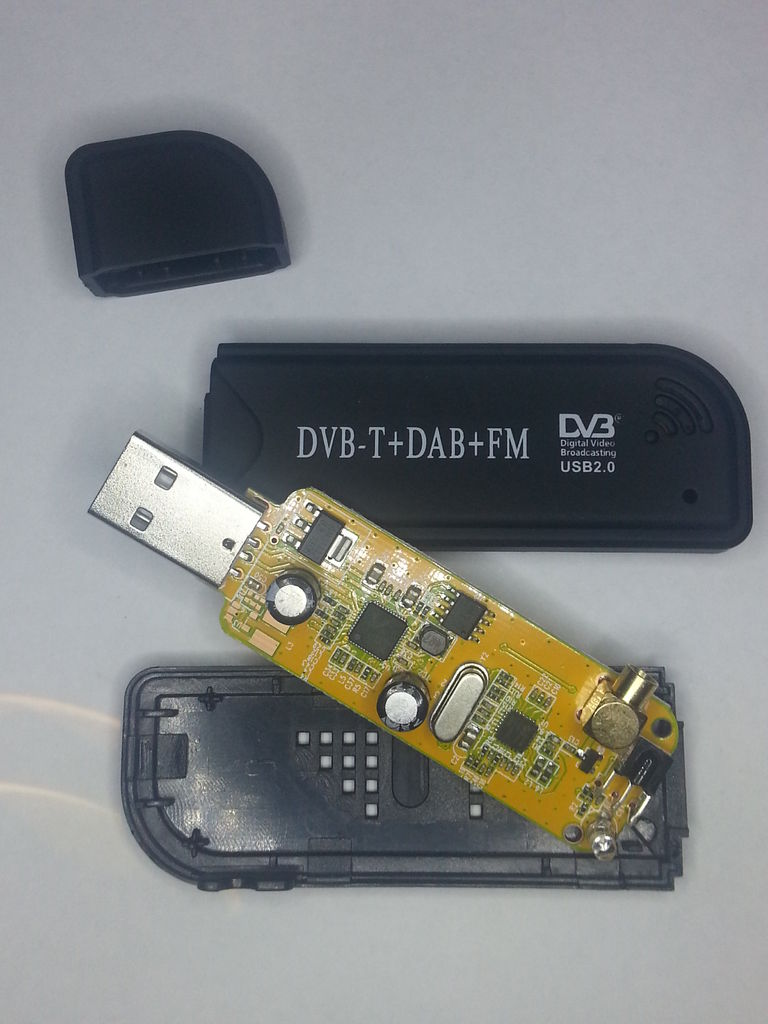
\includegraphics[width=0.5\textwidth]{SDR.jpg}
\par\end{centering}

\caption{Sintonizador de radio digital.}


\end{figure}



\subsection{Transmisión de TV por cable}

En telecomunicaciones, la televisión analógica se transmite mediante
el método de la Multiplexión por División en Frecuencia (FDM). Esta
técnica consiste en transmitir varias señales simultáneamente modulando
cada una con una portadora diferente, en el rango de VHF/UHF, de forma
tal que los anchos de banda de cada señal no se superpongan significativamente.
El canal destinado para la transmisión de una emisora tiene un ancho
de banda de aproximadamente 6 Mhz, donde los 5.45 Mhz más bajos corresponden
al espectro de la señal de video y los últimos 0.55Mhz (aproximadamente)
se reservan para el espectro de la señal de audio. Este modelo de
comunicación se puede ver representado en el siguiente gráfico:

\begin{figure}[H]
\begin{centering}
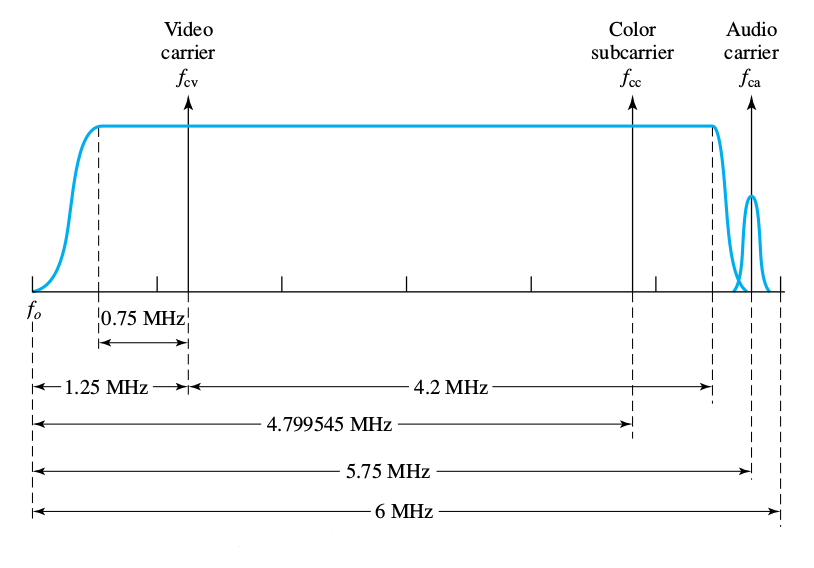
\includegraphics[width=0.75\textwidth]{TV_Spectrum.png}
\par\end{centering}

\caption{Señal de TV transmitida.}
\end{figure}



\subsection{Aplicación del Trabajo Práctico}

Sabiendo que el audio de la televisión está modulado en frecuencia
(FM), si se toma la porción del canal adecuada es posible demodular
dicha señal y escuchar algún canal de televisión.

En este caso particular, el SDR se utilizó para capturar un ancho
de banda de 2.4Mhz y centrado en 181.238 Mhz. A través del aplicativo
desarrollado se pudo escuchar efectivamente el programa emitido.


\section{Introducción}
Adoptamos la convención de code styling de Google para C++, salvando las siguientes excepciones:\\
\begin{itemize}
\item streams: utilizamos flujos de entrada y salida
\item sobrecarga de operadores
\item 

\end{itemize}
\section{Desarrollo}
\section{Códigos}
\section*{main.cc}
Los códigos no deben tener \textbf{\underline{texto acentuado}}.
\lstset{language=C++,%
    basicstyle=\color{red},
    breaklines=true,%
    morekeywords={matlab2tikz},
    keywordstyle=\color{blue},%
    morekeywords=[2]{1}, keywordstyle=[2]{\color{green}},
    identifierstyle=\color{black},%
    stringstyle=\color{mygreen},
    commentstyle=\color{mygray},%
    showstringspaces=false,%without this there will be a symbol in the places where there is a space
    numbers=left,%
    numberstyle={\tiny \color{mygray}},% size of the numbers
    numbersep=9pt, % this defines how far the numbers are from the text
    emph=[1]{for,end,break},emphstyle=[1]\color{blue}, %some words to emphasise
    emph=[2]{word1,word2}, emphstyle=[2]{style},    
}
\lstinputlisting{main.cc}

\end{document}